\documentclass[hidelinks, french]{article} %MAJ 1
\usepackage[a4paper, total={7in, 10in}]{geometry}
% get fontsized kido
\usepackage{fontsize}
  \changefontsize[14]{11}
\usepackage{amsmath}\usepackage{amssymb}\usepackage{mathcomp}

\usepackage[dvipsnames]{xcolor}\usepackage{mathrsfs}\usepackage{euscript}\usepackage{wasysym}[mathcal]\usepackage{stmaryrd}\usepackage{rsfso}
% pour les belles fonts
\usepackage{amsfonts}\usepackage{bbm} \DeclareMathAlphabet{\mathpzc}{OT1}{pzc}{m}{it}
% pour pouvoir utiliser les caractères accentués
\usepackage[utf8]{inputenc}
\usepackage[T1]{fontenc}
% pour les refs
\usepackage{cite}
% pour les beaux tableaux
\usepackage{multirow}
% pour gérer les figures
\usepackage{graphicx}
\usepackage{wrapfig}
% pour des matrices infernales
\usepackage{easybmat}
% pour rendre lien cliquable
\usepackage{hyperref}
% pour dessins et les diagrams
\usepackage{tikz}\usepackage{tikz-cd}
% pour les maxis graphs
\usepackage{scalerel}\usepackage{pict2e}\usepackage{tkz-euclide}
\usetikzlibrary{calc}\usetikzlibrary{patterns,arrows.meta} \usetikzlibrary{shadows}\usetikzlibrary{external}
% pour les maxis plots
\usepackage{pgfplots}\pgfplotsset{compat=newest}
\usepgfplotslibrary{statistics}\usepgfplotslibrary{fillbetween} \usepackage{nicefrac}
% pour la prog
\usepackage{fancyvrb}\usepackage{listings}
%\usepackage{algpseudocode}
% pour la prog -test-
\usepackage{pythontex}



%%%%    RACCOURCIS    %%%%
 
\newcommand{\N}{\mathbb{N}}
\newcommand{\Z}{\mathbb{Z}}   
\newcommand{\Q}{\mathbb{Q}}
\newcommand{\R}{\mathbb{R}}
\newcommand{\C}{\mathbb{C}}
\newcommand{\K}{\mathbb{K}}
\renewcommand{\k}{\Bbbk}
\newcommand{\U}{\mathbb{U}}
\renewcommand{\u}{\text{U}}
\newcommand{\A}{\mathbb{A}}
\newcommand{\T}{\mathscr{T}}
\newcommand{\I}{\mathbb{I}}
\newcommand{\F}{\mathcal{F}}
\renewcommand{\S}{\mathfrak{S}}
\newcommand{\matk}{\mathpzc{M}_n(\mathbb{K})}
\newcommand{\matr}{\mathpzc{M}_n(\mathbb{R})}
\newcommand{\lr}{\longrightarrow}
\newcommand{\Lr}{\Longrightarrow}
\renewcommand{\ll}{\longleftarrow}
\newcommand{\Ll}{\Longleftarrow}
\newcommand{\llr}{\longleftrightarrow}
\newcommand{\Llr}{\Longleftrightarrow}
\newcommand{\para}{\sslash}
\newcommand{\Arccos}{\text{Arccos}} 
\newcommand{\Arcsin}{\text{Arcsin}} 
\newcommand{\Arctan}{\text{Arctan}} 
\newcommand{\Argch}{\text{Argch}}       
\newcommand{\Argsh}{\text{Argsh}}
\newcommand{\pgcd}{\text{pgcd}}
\newcommand{\PGCD}{\text{PGCD}}
\newcommand{\ppmc}{\text{ppcm}}
\newcommand{\sign}{\text{sign}}
\renewcommand{\Vec}{\text{Vec}}
\newcommand{\Aff}{\text{Aff}}
\newcommand{\sgn}{\text{sgn}}
\newcommand{\Deg}{\text{Deg}}
\newcommand{\ord}{\text{ord}}
\renewcommand{\det}{\text{det}}
\newcommand{\Ker}{\text{Ker}}
\newcommand{\Ann}{\text{Ann}}
\newcommand{\codim}{\text{codim}}
\newcommand{\tr}{\text{tr}}
\newcommand{\rg}{\text{rg}}
\newcommand{\Co}{\text{com}}
\newcommand{\Sp}{\text{Sp}} 
\newcommand{\GL}{\text{GL}}
\newcommand{\GA}{\text{GA}}
\newcommand{\SL}{\text{SL}}
\newcommand{\SO}{\text{SO}}
\newcommand{\HT}{\text{HT}}
\newcommand{\im}{\text{Im}}
\renewcommand{\div}{\text{div}}
\newcommand{\rot}{\text{rot}}
\renewcommand{\O}{\varnothing}
\renewcommand{\epsilon}{\varepsilon}
\renewcommand{\subsetneq}{\varsubsetneq}
\renewcommand{\leq}{\leqslant}
\renewcommand{\geq}{\geqslant}
\renewcommand{\AC}{\sim}
\renewcommand{\limsup}{\varlimsup}
\renewcommand{\liminf}{\varliminf}
\renewcommand{\stop}{\text{\;{\scriptsize$\top$}\;}}
\newcommand{\sbot}{\text{\;{\scriptsize$\bot$}\;}}
% Avec Paramètre
\newcommand{\argmin}[1]{\underset{#1}{\text{argmin}}}
\newcommand{\argmax}[1]{\underset{#1}{\text{argmax}}}
\newcommand{\Top}[1]{\underset{#1}{\ \text{\huge{$\top$}}}\ }
\newcommand{\Topp}[2]{\ \underset{#1}{\overset{#2}{\text{\huge{$\top$}}}}\ }
\newcommand{\Bot}[1]{\underset{#1}{\ \text{\huge{$\bot$}}}\ }
\newcommand{\Bott}[2]{\ \underset{#1}{\overset{#2}{\text{\huge{$\bot$}}}}\ }





% set up des captions figures (extrêmement BG) :
\usepackage{subcaption}
\usepackage{floatrow}
\captionsetup{justification=centering}
\DeclareCaptionLabelFormat{custom}{\textit{fig. #2}}
\DeclareCaptionLabelSeparator{custom}{\, ---\, }
\DeclareCaptionFormat{custom}{#1#2#3}
\DeclareCaptionFont{custom}{\itshape }
\renewcommand{\thefigure}{\arabic{figure}}
\newcommand{\figref}[1]{\textit{fig. \ref{#1}}}
\pgfplotsset{standard/.style={width=0.4\textwidth,
    height=0.2\textwidth,
    compat=1.18,
    trig format=rad,
    enlargelimits,
    enlarge x limits=0.05,
    enlarge y limits=0.05,
    every axis x label/.style={footnotesize, at={(current axis.right of origin)},anchor=north west},
    every axis y label/.style={footnotesize, at={(current axis.above origin)},anchor=south east},
    scale only axis=true}}

\begin{document}
\begin{figure}[H]\centering
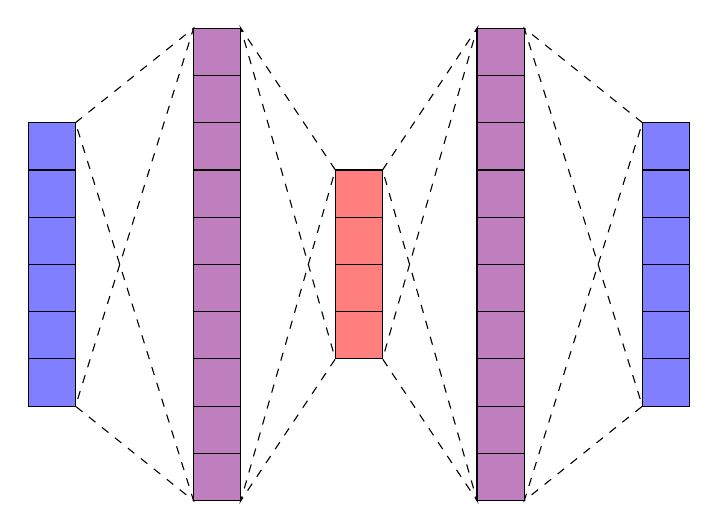
\begin{tikzpicture}[scale=0.6]
%\draw[thin, opacity=0.5] (-7.5,-6.5) grid (7.5,6.5);

%%% vecteurs

% input
\draw[fill=blue, fill opacity=0.5] (-7,-3) -- (-7,3) -- (-6,3)  -- (-6,-3) -- (-7,-3);
\draw (-7, 2) -- (-6, 2);
\draw (-7, 1) -- (-6, 1);
\draw (-7, 0) -- (-6, 0);
\draw (-7, -1) -- (-6, -1);
\draw (-7, -2) -- (-6, -2);

% hidden 1
\draw[fill=violet, fill opacity=0.5] (-3.5,-5) -- (-2.5,-5) -- (-2.5,5)  -- (-3.5,5) -- (-3.5,-5);
\draw (-3.5, 4) -- (-2.5, 4);
\draw (-3.5, 3) -- (-2.5, 3);
\draw (-3.5, 2) -- (-2.5, 2);
\draw (-3.5, 1) -- (-2.5, 1);
\draw (-3.5, 0) -- (-2.5, 0);
\draw (-3.5, -1) -- (-2.5, -1);
\draw (-3.5, -2) -- (-2.5, -2);
\draw (-3.5, -3) -- (-2.5, -3);
\draw (-3.5, -4) -- (-2.5, -4);

% latent
\draw[fill=red, fill opacity=0.5] (-0.5,-2) -- (0.5,-2) -- (0.5,2)  -- (-0.5,2) -- (-0.5,-2);
\draw (-0.5, 1) -- (0.5, 1);
\draw (-0.5, 0) -- (0.5, 0);
\draw (-0.5, -1) -- (0.5, -1);

% hidden 2
\draw[fill=violet, fill opacity=0.5] (3.5,-5) -- (2.5,-5) -- (2.5,5)  -- (3.5,5) -- (3.5,-5);
\draw (3.5, 4) -- (2.5, 4);
\draw (3.5, 3) -- (2.5, 3);
\draw (3.5, 2) -- (2.5, 2);
\draw (3.5, 1) -- (2.5, 1);
\draw (3.5, 0) -- (2.5, 0);
\draw (3.5, -1) -- (2.5, -1);
\draw (3.5, -2) -- (2.5, -2);
\draw (3.5, -3) -- (2.5, -3);
\draw (3.5, -4) -- (2.5, -4);

% output
\draw[fill=blue, fill opacity=0.5] (7,-3) -- (7,3) -- (6,3)  -- (6,-3) -- (7,-3);
\draw (7, 2) -- (6, 2);
\draw (7, 1) -- (6, 1);
\draw (7, 0) -- (6, 0);
\draw (7, -1) -- (6, -1);
\draw (7, -2) -- (6, -2);

%%% vecteurs

% links1
\draw[dashed, thin] (-6,3) -- (-3.5,5) -- (-6,-3) -- (-3.5,-5) -- (-6,3);
\draw[dashed, thin] (-0.5,2) -- (-2.5,5) -- (-0.5,-2) -- (-2.5,-5) -- (-0.5,2);
\draw[dashed, thin] (0.5,2) -- (2.5,5) -- (0.5,-2) -- (2.5,-5) -- (0.5,2);
\draw[dashed, thin] (6,3) -- (3.5,5) -- (6,-3) -- (3.5,-5) -- (6,3);


\end{tikzpicture}
    \caption{a caption}
    \label{fig:enter-label}
\end{figure}

\end{document}